\chapter{Main Entities} \label{chap:entities}

 \NOTE{This description has not been updated for ViennaGrid 1.1.0 yet!}
 

In the following, the main entities of ViennaGrid are explained. The nomenclature essentially follows the convention from topology and can partly be found in other mesh libraries. Note that the purpose of this manual is not to give exact definitions from the field of geometry or topology, but rather to establish the link between abstract concepts and their representation in code within {\ViennaGrid}. First, geometrical objects are discussed, then topological objects and finally complexes of topological objects.

\begin{figure}[tb]
\centering
 \fbox{ 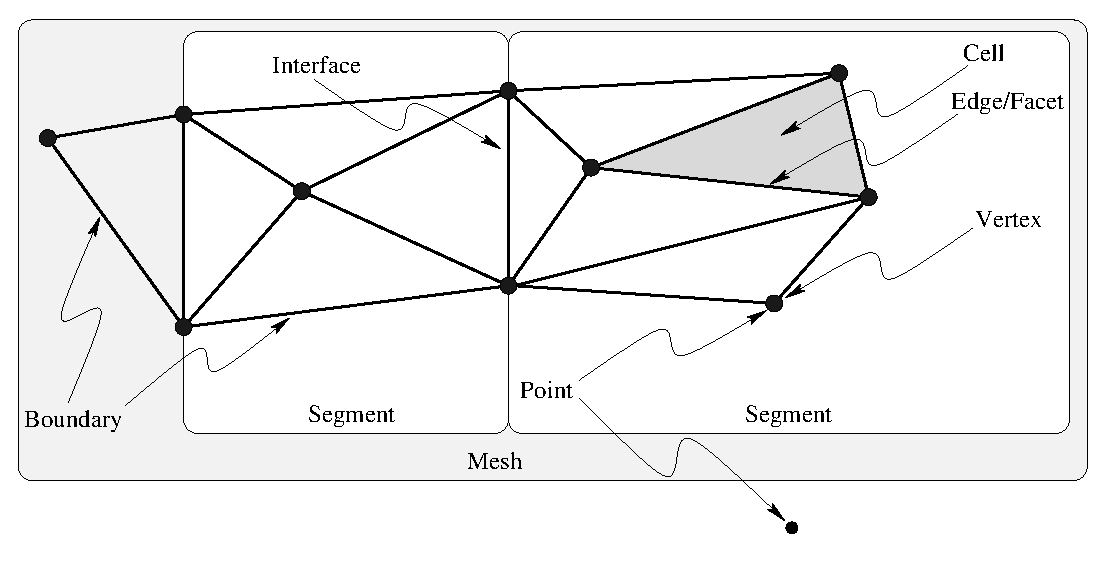
\includegraphics[width=0.95\textwidth]{figures/entities.eps} }
 \caption{Overview of the main entities in {\ViennaGrid} for a triangular mesh. A point refers to any location in the geometric space and does not carry topological information.}
 \label{fig:entities}
\end{figure}


\section{Points (Geometrical Objects)}
The underlying space in {\ViennaGrid} is the $m$-dimensional Euclidian space $\mathbb{E}^m$, which is identified with the real coordinate space $\mathbb{R}^m$ in the following.
A \emph{point} refers to an element $\vector x$ in $\mathbb{R}^m$ and does not carry any topological information. On the other hand, a point equivalently refers to the vector from the origin pointing to $\vector x$.

Given a configuration class \lstinline|Config| for {\ViennaGrid} (cf.~Chap.~\ref{chap:domainconfig}), a point is defined and manipulated as follows:
\begin{lstlisting}
 using namespace viennagrid;

 // obtain the point type from a meta-function
 typedef result_of::point<Config>::type    PointType;
 // For a three-dimensional Cartesian space (double precision),
 // the type of the point is returned as
 // point_t<double, cartesian_cs<3> >

 // Instantiate two points:
 PointType p1(0, 1, 2);
 PointType p2(2, 1, 0);

 // Add/Subtract points:
 PointType p3 = p1 + p2;
 std::cout << p1 - 2.0 * p3 << std::endl;
 std::cout << "x-coordinate of p1: " << p1[0] << std::endl;
\end{lstlisting}
The operators \lstinline|+, -, *, /, +=, -=, *=| and \lstinline|/=| can be used in the usual mnemonic manner. \lstinline|operator[]| grants access to the individual coordinate entries and allows for a direct manipulation.

Aside from the standard Cartesian coordinates, {\ViennaGrid} can also handle polar, spherical and cylindrical coordinate systems.
This is typically defined globally within the configuration class \lstinline|Config| for the whole domain, and the meta-function in the previous snippet creates the correct point type. However, if no global configuration class is available, the point types can be obtained as
\begin{lstlisting}
 typedef point<double, 1>                   CartesianPoint1d;
 typedef point<double, 2>                   CartesianPoint2d;
 typedef point<double, 2, polar_cs>         PolarPoint2d;
 typedef point<double, 3>                   CartesianPoint3d;
 typedef point<double, 3, spherical_cs>     SphericalPoint3d;
 typedef point<double, 3, cylindrical_cs>   CylindricalPoint3d;
\end{lstlisting}
Conversions between the coordinate systems are carried out implicitly whenever a point is assigned to a point with a different coordinate system:
\begin{lstlisting}
 CylindricalPoint3d p1(1, 1, 5);
 CartesianPoint3d p2 = p1; //implicit conversion
\end{lstlisting}
An explicit conversion to the Cartesian coordinate system is provided by the free function \lstinline|to_cartesian()|, which allows for the implementation of generic algorithms based on Cartesian coordinate systems without tedious dispatches based on the coordinate systems involved.

\TIP{For details on the coordinate systems, refer to the reference documentation in \texttt{doc/doxygen/}.}

Since all coordinate systems refer to a common underlying Euclidian space, the operator overloads remain valid even if operands are given in different coordinate systems. In such a case, the coordinate system of the resulting point is given by the coordinate system of the left hand side operand:
\begin{lstlisting}
 CylindricalPoint3d p1(1, 1, 5);
 CartesianPoint3d p2 = p1; //implicit conversion

 // the result of p1 + p2 is in cylindrical coordinates
 CylindricalPoint3d p3 = p1 + p2;

 // the result of p2 + p1 is in Cartesian coordinates,
 // but implicitly converted to cylindrical coordinates:
 CylindricalPoint3d p4 = p2 + p1;
\end{lstlisting}
For additional algorithms acting on points, e.g.~\lstinline|norm()| for computing the norm/length of a vector, please refer to Chapter \ref{chap:algorithms}.

\TIP{ViennaGrid is not restricted to one, two or three geometric dimensions! Cartesian coordinate systems for arbitrary dimensions are available.}

\section{Elements (Topological Objects)} \label{sec:ncells}
While the point type defines the underlying geometry, elements define the topological connections among distinguished points. Each of these distinguished points is called a \emph{vertex} and describes the corners or intersection of geometric shapes. Vertices are often also referred to as the \emph{nodes} of a mesh.

An \emph{edge} or \emph{line} is a line segment joining two vertices. Note that this is a topological characterization -- the underlying geometric space can have arbitrary dimension.

A \emph{cell} is an element of maximum topological dimension $N$ within the set of elements considered. The topological dimension of cells can be smaller than the underlying geometric space, which is for example the case in triangular surface meshes in three dimensions. Note that the nomenclature used among scientists is not entirely consistent: Some refer to topologically three-dimensional objects independent from the topological dimension of the full mesh as cells, which is not the case here. 

The surface of a cell consists of \emph{facets}, which are objects of topological dimension $N-1$. Some authors prefer the name \emph{face}, which is by other authors used to refer to objects of topological dimension two. Again, the definition of a facet refers in {\ViennaGrid} to topological dimension $N-1$.

Boundary elements are elements which represent a boundary of another element. For example a triangle is a boundary element of a tetrahedron. But not only the direct boundaries are boundary elements in {\ViennaGrid}, also a boundary element of boundary element of an element is a boundary element of that element: a vertex and a line is a boundary element of a tetrahedron as well.

\begin{table}[b]
 \centering 
 \renewcommand{\arraystretch}{1.3}
\begin{tabular}{|l|l|l|l|l|}
\hline
          &  $1$-d & $2$-d & $3$-d & $n$-d \\
\hline
 \textbf{Vertex}   & Point  & Point & Point & Point \\
 \textbf{Edge}     & Line   & Line  & Line  & Line \\
 \textbf{Facet}   & Point  & Line  & Triangle, etc. & $n-1$-Simplex, etc. \\
 \textbf{Cell}   & Line   & Triangle, etc. & Tetrahedron, etc. & $n$-Simplex \\
\hline
\end{tabular}
\caption{Examples for the vertices, edges, facets and cells for various topological dimensions.}
\label{tab:vertex-edge-facet-cell}
\end{table}

A brief overview of the corresponding meanings of vertices, edges, facets and cells is given in Tab.~\ref{tab:vertex-edge-facet-cell}. Note that edges have higher topological dimension than facets in the one-dimensional case, while they coincide in two dimensions. Refer also to Fig.~\ref{fig:entities}.

% For a parametric description of these objects it is more appropriate to switch \textbf{$n$-cells}, which are objects of topological dimension $n$. The terms \emph{vertex}, \emph{edge}, \emph{facet} and \emph{cell} thus refer to $0$-cell, $1$-cell, $N-1$-cell and $N$-cell respectively. The maximum topological dimension $N$ is in {\ViennaGrid} considered to be a parameter available at compile time, which allows to pick the correct $n$-cell type for the algorithms provided. Note that one can still use a run time dispatch at the cost of increased compilation times if the dimension of the domain is only available at run time. More details can be found in Chapters \ref{chap:iterators} and \ref{chap:algorithms}.


\section{Domain}
A \emph{domain} $\Omega$ is the top level object in {\ViennaGrid} and is a container for its topological elements. There are no topological restrictions on the elements inside a domain. 

A typical use-case for a domain is to store a cell complex. We characterize a cell complex as a collection of topological elements, such that the intersection of two elements (maybe of different type) $e_0$ and $e_1$  is another element $e_i$ from the cell complex.

It should be noted that {\ViennaGrid} allows the use of conforming and non-conforming complexes. Here, a \emph{conforming} complex is characterized by the property that the intersection element $e_i$  from above is a boundary element from both of the element $e_0$ and the element $e_1$.

If this is not the case, the complex is denoted \emph{non-conforming}, cf.~Fig.~\ref{fig:conformity}.

\begin{figure}[tb]
\centering 
   \subfigure[Conforming cell complex.]{
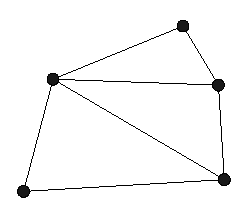
\includegraphics[width=0.23\textwidth]{figures/conforming.eps}
} \hspace*{2cm}
   \subfigure[Non-conforming cell complex.]{ \label{subfig:non-conforming}
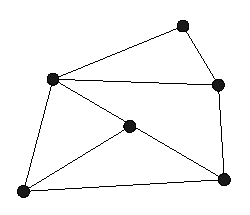
\includegraphics[width=0.23\textwidth]{figures/non-conforming}
 }
 \caption{Illustration of conforming and non-conforming cell complexes. The vertex in the center of \subref{subfig:non-conforming} intersects an edge in the interior, violating the conformity criterion.}
 \label{fig:conformity}
\end{figure}

The instantiation of a {\ViennaGrid} domain object requires a configuration class \lstinline|Config|, as will be discussed in~Chapter~\ref{chap:domainconfig}. Given such a class, the domain type is retrieved and the domain object constructed as 
\begin{lstlisting}
 using namespace viennagrid;

 // Type retrieval, method 1: use meta-function (recommended)
 typedef result_of::domain<Config>::type     DomainType;

 // Type retrieval, method 2: direct (discouraged, may change in future versions)
 typedef domain_t<Config>     DomainType

 DomainType domain; //create the domain object
\end{lstlisting}

\section{Segmentation and Segment}
A \emph{segment} $\Omega_i$ refers to a subset of the elements in a domain $\Omega$. Unlike a domain, a segment is not a container for its elements. Instead, only references (pointers) to the elements in the domain are stored. In common C++ language, a \emph{segment} represents a so-called \emph{view} on the domain.

A segmentation represents a collection of segments. The typical use-case for a segmentation is the decomposition of the domain into pieces of a common property. For example, a solid consisting of different materials can be set up in {\ViennaGrid} such that each regions of the same material are represented in a common segment.


